\chapter{Causal Networks with Neural Networks}

\section{Introduction}\label{S:2.1}

The causal network of a dynamical system provides important information that may help to better understand its behavior and ultimately design better policies to predict and control it. 
Large number of banks, insurances, hedge funds, and other financial institutions around the globe are interacting daily and thus their causal network is of great importance in econometrics.  

There have been many attempts during the past decades to capture and visualize the network of interconnections among a set of financial institutions. 
A well-known time series causality measure used in econometrics is Granger-causality (\citet{granger}).
This is based on statistical analysis of the financial time series such as their stock prices over a finite time period. 
Granger’s definition of causality states that a time serie $X$ is a cause of another time serie $Y$, if the one-step future forecast of $Y$ is more precise when the forecasting information set includes X. 
Otherwise, when the forecast does not improve by including the information of $X$, then it is declared that $X$ does not cause $Y$.
This idea is reflected in the information-theoretic measure that we use in this chapter to infer the causal interactions among a network of time series.  

Most empirical applications of Granger-causality have been studied with Vector Autoregressive (VAR) models. 
For instance, \citet{billio2012econometric} propose several measures based on Granger-causality to capture the interconnections between the returns of financial institutions on a monthly basis. 
It uses principle component analysis and pairwise Granger-causality tests to identify the causal networks. 
Other related works are \citet{diebold2014network} and \citet{barigozzi2016network} in which the authors propose connectedness measures based on generalized variance decomposition.
However, the measures introduced in these works are again limited to linear systems and they are based on pairwise comparison which as we show in Section  \ref{sec:dig} fails to infer the true causal relationships.
%and they are based on pairwise comparison which as we show in Section \ref{sec:dig}, it fail to infer the true causal relationships.
 %focuses on one particular network structure: the long-run variance decomposition network. Such networks are characterized by the infinite vector moving average and similar to \citet{diebold2014network}, they are limited to linear systems.

\clearpage
Contributions of this chapter are both in network identification literature and in finance.
%This paper adds contribution in the network identification literature as well as in finance literature. 
Our contributions to network identification are as follows:
\begin{itemize}
    \item We use directed information (DI), an information measure to infer the Granger-causalities among a set of time series. 
This measure is non-parametric (i.e. it does not depend on the underlying model of the dynamics) and it is capable of capturing causal relationships in both linear and nonlinear systems. The output of this approach is a directed graph known as Directed Information Graph (DIG) that visualizes the interconnections among a set of time series such as stock returns. 

\item Computing DI has high computational and sample complexity which makes it not suitable for inferring the causal structure of large networks. 
To solve this problem, we develop a novel approach based on Recurrent Neural Networks (RNNs) that reduces the complexity of evaluating DIs in high-dimensional settings. 
\end{itemize}


%show that Directed Information is biased when the information set does not include all true parents, resulting in an imprecise network graph. To overcome this issue, we develop an algorithm to consistently estimate Directed Information while reducing complexity. 

Applications of DIG are various in finance. 
In particular, we recommend to use it as a preliminary feature selection of another predictive model. Feature selection is a process often used in machine learning and statistics which consists of keeping only a subset of relevant features, usually to avoid overfitting or to reduce dimensionality. 
For example, \citet{fs1} and \citet{fs2} show that extraneous features are prone to reduce model's performance measures. 
Finance applications of feature selection models are various and include credit scoring, stock market behavior analysis  or even fraud detection (\citet{fs_fraud}).
\citet{tsai2009} states that feature selection preprocessing is not addressed carefully enough in the bankruptcy prediction literature. They compare five feature selection methods used in bankruptcy prediction: step-wise regressions, correlation matrix, principal component analysis, t-tests and factor analysis and show that any of these methods improves performance. 
\citet{fs_stock} uses a Sequential Forward Selection algorithm to select relevant features predicting the Turkish market index. The use of such feature selection model reduces model prediction error compared to the case where all features are used. This is due to information embedded in several economic factors already included in the market index. 

%In this work, we use an information-theoretic measure known as directed information (DI) to infer the Granger-causalities among a set of time series. 
%This measure does not depend on the underlying model of the dynamic and it is capable of capturing causal relationships in both linear and nonlinear systems.
%However, computing DI has both high computational and sample complexity which makes it not suitable for inferring the causal structure of large networks. 
%To overcome this problem, we develop a novel approach based on Recurrent Neural Networks (RNNs) that reduces the complexity of evaluating DIs in high-dimensional settings. 

\subsection{Related Work}
In recent years, several approaches have been developed to generalize the applicability of Granger-causality to non-linear and large dynamics. 
To mention a few, \citet{psaradakis2005markov} introduce different terminologies for causality based on Granger’s ideas and provide a set of parametric non-causality constraints in the context of Markov switching VAR models.
In a similar context, \citet{bianchi2019modeling} investigate time-varying systemic risk based on a range of multi-factor asset pricing models and develop a Markov Chain Monte Carlo scheme to infer their model parameters and consequently obtain their corresponding networks.
Another attempt is \citet{bonaccolto2019estimation} in which the authors explore quantile-based methods of Granger-causality.
%This work focuses on the linear factor model augmented with network dependence introduced by \citet{billio2018networks} and develops a method to identify causality among quantiles of the time series. 
This method is consistent with \citet{hong2009granger} and \citet{corsi2018measuring} that focus on causality among tail events. 
These methods are suitable for capturing causal relationships that are not in the center of their distributions, or in the mean but in the tails of their distributions.
It is important to emphasize that our proposed approach using DI is also capable of capturing such causal relations. 

Most of the above aforementioned approaches are developed and tested for small size networks. 
Often, the problem of network identification in high dimensional settings requires more considerations and even its own techniques. 
For instance, \citet{billio2019bayesian} propose a Bayesian non-parametric Lasso (BNPL) prior for high-dimensional vector autoregressive models that improve efficiency and accuracy. 
To overcome overfitting in large VAR models, BNPL clusters the vector autoregressive coefficients and shrinks the coefficients of each cluster toward a common location.
%Although, the proposed method in this work is suitable for inference in high dimensional VAR models but 
However, this method is limited to linear models with Gaussian innovations.
To overcome this limitation, \citet{kalli2018bayesian} propose a Bayesian non-parametric approach that allows for nonlinearity in the conditional mean, heteroskedasticity in the conditional variance, and non-Gaussian innovations. However, unlike the BNP-Lasso, it does not allow sparsity in the model.
\citet{petrova2019quasi} proposes yet another non-parametric, quasi-Bayesian likelihood estimation methodology for high dimensional setting with time-varying parameters. 
%This method is also non-parametric. 
The work in \citet{iacopini2019bayesian} tackles the curse of dimensionality by a two-stage approach. First, a spike-and-slab prior distribution is used for each entry of the coefficient matrix which also identifies the interconnection network.
In the second stage, it imposes prior dependence on the coefficients by specifying a Markov process for their random distribution. 
%A side product of this procedure is the interconnection network.
A closely related work is \citet{bernardi2019high} that proposes a shrinkage and selection methodology designed for network inference in high-dimensional settings. It uses a regularized linear regression model with spike-and-slab prior on the parameters.
However, both methods are limited to VAR models.



The remainder of this chapter is strutured as follows. 
Section \ref{Sec1} reviews the notion of Granger-causality and formally introduces directed information graphs which are suitable for linear and nonlinear systems. 
Section \ref{sec:method} introduces a novel approach for inferring the Granger-causal network of high dimensional nonlinear systems. 
Section \ref{sec:exp} applies our methodology to learn the causal network of both synthetic and real-world dataset. For the real-world experiment, we use the daily stock prices of US firms.

%Afterwards, we evaluate the performance of our method in both synthetic linear and nonlinear settings and also apply it to infer the interconnections among the major US financial institutions.


\section{Causal Network}\label{Sec1}

We present in this section our econometric approach to learn the causal dependencies in a dynamical systems based on Granger-causality (see \citet{granger}). 
We begin by introducing some notations.
Plain capital letters denote random variables or processes, while lowercase letters denote their realizations. 
Bold letters are used for column vectors, matrices, and tensors and calligraphy letters are used for sets. 
We use $X_{j,t}$ to denote the value of a time series $X_j$ at time $t$ 
%and $X_{j,t_1}^{t_2}$, when $t_1\leq t_2$, to denote $X_j$ from time $t_1$ to $t_2$, namely, $(X_{j,t_1},...,X_{j,t_2})$. 
%Subsequently, 
and $X^{t}_j$ to denote the time series $X_j$ up to time $t$. 
For a set $\mathcal{A}=\{a_1,...,a_n\}$ and an index set $\mathcal{I}\subseteq\{1,...,n\}$, we define $\mathcal{A}_{-\mathcal{I}}:=\mathcal{A}\setminus\{a_i: i\in\mathcal{I}\}$. 



\subsection{Granger Causality}\label{sec:granger}

Various frameworks and graphical models have been developed to capture and represent interconnections among variables or processes.
One of the most popular and widely used frameworks in economics is the notion of Granger-causality originally introduced by \citet{wiener1956theory} and
generalized by \citet{granger}. We say that $X$ Granger-causes $Y$ if the prediction of the future of $Y$ is more precise using all available information (including $X$) than using all available information except $X$.

This formulation was originally implemented using multivariate autoregressive (MVAR) models and linear regressions.
In particular, let $\{X,Y,Z\}$ be three time series. In order to identify the influence of $X_t$ on $Y_t$, Granger's idea is to compare the performance of two linear regressions\footnote{Note that this formulation is only applicable in linear systems.}: the first one predicts $Y_t$ given $\{X^{t-1},Y^{t-1},Z^{t-1}\}$ and the second one predicts $Y_t$ given $\{Y^{t-1},Z^{t-1}\}$. If they perform similarly, then we say $X$ does not Granger-cause $Y$.

To go beyond linear systems, works such as \citet{directed} and \citet{massey} use information-theoretical measures and generalize Granger-causality. 
In this chapter, we introduce and apply directed information (see \citet{directed}), an information-theoretical tool to measure interconnections among firms.
Directed information (DI) has been used in many applications to infer causal relationships. For example, \citet{spike} and \citet{di12} use it for analyzing neuroscience data and \citet{acc2014}  and \citet{etesami2018econometric} apply it to market data. 


Directed information graphs (DIGs) have been developed to visualize the inferred interconnections among time series (see \citet{directed}).  
DIGs are a type of graphical models in which nodes represent time series and arrows indicate the direction of causation. We use DIG to represent the causal network among the covered firms. 



\subsection{Directed Information Graphs (DIGs)}\label{sec:dig}


We describe in this section how the directed information is able to capture the connections in causal networks. Next, we formally define directed information graphs (DIG).

We define a dynamical system constituted of three time series $\{X,Y,Z\}$ that we assume have a joint probability density function $p(X,Y,Z)$. 
Granger-causality states that to know whether $X$ influences $Y$ or not, we need to compare the performance of two predictors of $Y$.
The first predictor uses the history of all information available (i.e. $\{X,Y,Z\}$) while the second predictor uses only the history of $\{Y,Z\}$
If the former performs better than the latter, $X$ has information on $Y$. However, if they perform equally, it is an indication that $X$ is not causing $Y$ in this time interval.
To rigorously formalize this idea, we need the predictors and a measure to compare their performances.

\clearpage

In the definition of DI,  the predictors belong to the space of probability measures.  
More precisely,  
%let $X^{t-1}$ represents the time series $X$ up to time $t-1$.
the prediction of the first predictor at time $t$ is $p(Y_t|Y^{t-1},Z^{t-1},X^{t-1})$ that is the conditional density function of $Y_t$ given the history of all time series. Similarly, the prediction of the second predictor is $p(Y_t|Y^{t-1},Z^{t-1})$ that is the conditional density function of $Y_t$ given the history of all time series except time series $X$.

Given the predictions of the first and the second predictors at time $t$ for an outcome $y_t\in \mathcal{Y}$, the goodness of these predictions are measured by the log-loss that are defined respectively by 
\begin{align*}
    &-\log p(Y_t=y_t|Y^{t-1},Z^{t-1},X^{t-1}),\\
    &-\log p(Y_t=y_t|Y^{t-1},Z^{t-1}).
\end{align*}
According to the above measures of goodness, the better the predictor is, the smaller its log-loss will be.
This loss function also has meaningful information-theoretical interpretations.
Namely, the log-loss is the Shannon's code length\footnote{It is also called the description length of $y_t$. For more information see \citet{cover2012elements}.}, i.e., the number of bits required to efficiently represent $y_t$ (see \citet{etesami2018econometric}). 

At time $t$ for an outcome $y_t\in \mathcal{Y}$, the difference between the log-losses of the two predictors compares their performances.  This difference is also called regret, denoted $r_t$ :
\begin{align}
r_t:&=-\log{p(Y_t=y_t|Y^{t-1},Z^{t-1})}-\big(-\log {p(Y_t=y_t|Y^{t-1},Z^{t-1},X^{t-1})}\big) \nonumber \\
&=\log \frac{p(Y_t=y_t|Y^{t-1},Z^{t-1},X^{t-1})}{p(Y_t=y_t|Y^{t-1},Z^{t-1})}.
\end{align}
Regrets are always positive for all $t$ and all outcomes $y_t$.
Over the time interval $[1,T]$, the average regret is
\begin{align}\label{eq:ave}
   \frac{1}{T}\sum_{t=1}^T \mathbb{E}[r_t],
\end{align}
where the expectation is taken over the joint density function\footnote{For the sake of notational simplicity, we use $p(y^{t},z^{t-1},x^{t-1})$ to denote $p(Y^{t}=y^{t},Z^{t-1}=z^{t-1},X^{t-1}=x^{t-1})$.} of $X$, $Y$, and $Z$, i.e., 
\begin{align}
    \mathbb{E}[r_t]=\int p(y^{t},z^{t-1},x^{t-1})\log \frac{p(y_t|y^{t-1},z^{t-1},x^{t-1})}{p(y_t|y^{t-1},z^{t-1})}dy^tdx^{t-1}dz^{t-1}.
\end{align}
The average regret in \eqref{eq:ave} is the directed information (DI). We use it as the measure of causation in this chapter.
This measure is always positive and if it is zero, it is an indication that the history of the time serie $X$ does not contain significant information helping in the prediction of the time serie $Y$ given the past of the time series $Y$ and $Z$. 
We can generalize this definition to more than three time series as follows,

\clearpage

 \begin{definition}\label{cdi}
Consider a network of $m$ time series $\mathcal{R}=\{R_1,...,R_m\}$ with the joint probability density function $p$. The directed information from $R_i$ to $R_j$ over the time interval $[1,T]$ is given by
\begin{align}\label{cdif}
I(R_i\rightarrow R_j||\mathcal{R}_{-\{i,j\}}):=\frac{1}{T}\sum_{t=1}^T\mathbb{E}\left[\log\frac{p(R_{j,t}|\mathcal{R}^{t-1}_{-\{i,j\}},R_{j}^{t-1},R_{i}^{t-1})}{p(R_{j,t}|\mathcal{R}^{t-1}_{-\{i,j\}},R_{j}^{t-1})}\right],
\end{align}
where $\mathcal{R}_{-\{i,j\}}^{t-1}\!:=\!\{R_{1}^{t-1},...,R_{m}^{t-1}\}\!\setminus\!\{R_{i}^{t-1},R_{j}^{t-1}\}$.
We say that $R_i$ has influence on $R_j$ over the time interval $[1,T]$, if and only if
\begin{align}\label{cdif1}
I(R_i\rightarrow R_j||\mathcal{R}_{-\{i,j\}})>0.
\end{align}
 \end{definition}
 
An interpretation of $R_i$ influencing $R_j$ is that varying $R_i$ will change the value of $R_j$ even if all the other variables within the network remains unchanged. 
 In another words, if $R_i$ does not influence $R_j$, then varying $R_i$ would not change $R_j$ when the values of the remaining times series are fixed. 
 This can be seen from the fact that DI compares two conditional distributions of $R_j$ over a time horizon of length $T$; one is conditioned on the past of all time series while the other one is conditioned on all the history except $R_i$. Thus, if DI in \eqref{cdif} is zero, then these two conditional distributions are equal over this time horizon. This implies that the history of $R_i$ does not contain any useful information for $R_j$.  
 
 
Note that the definition of DI does not rely on any model assumption, thus DI is capable of inferring the causal relationships in general (linear or non-linear) dynamical systems. Next, we define the graphical model that we use in this chapter to visualize the causal network among firms.


\begin{definition}\label{DIG1}
We denote by DIG the directed information graph of a set of $m$ time series $\mathcal{R}=\{R_1,...,R_m\}$ which consists of a directed graph $G=(\mathcal{V},\mathcal{E})$, where $\mathcal{V}$ stands for the set of nodes representing time series $\mathcal{R}$ while $\mathcal{E}$ stands for the set of arrows indicating influences between time series (i.e. an arrow from $R_i$ to  $R_j$ indicates that $R_i$ has an influence on $R_j$). 
%with weight $w_{i,j}:=I(R_i\rightarrow R_j||\mathcal{R}_{-\{i,j\}})$. 
%Consequently, $(R_i,R_j)\notin \mathcal{E}$ if and only if its corresponding weight is zero.
\end{definition} 

A simple way to represent the DIG $G$ of a dynamical system is via the adjacency matrix $\textbf{DIG}=[d_{i,j}]_{m\times m}$ that is defined by
\begin{align}
    d_{j,i} = \left\{
\begin{array}{ll}
      1 & \text{if}\  I(R_i\rightarrow R_j||\mathcal{R}_{-\{i,j\}})>0,\\
      0 & \text{otherwise}. \\
\end{array} 
\right. 
\end{align}
Given a DIG $G=(\mathcal{V},\mathcal{E})$, we define the parent set of node $R_j$ denoted by $\mathcal{PA}_j\subset \mathcal{V}$ to be the set of all times series that have direct influences on $R_j$, i.e., $\mathcal{PA}_j:=\{R_k: d_{j,k}=1\}$. Similarly, the children set of node $R_j$ is given by $\mathcal{CH}_j:=\{R_k: d_{k,j}=1\}$. 
Example \ref{r1} demonstrates the DIG of a simple linear system.

\clearpage

\begin{example}\label{r1}
Let $\{X,Y,Z\}$ be a network of three time series with the following dynamics,
\begin{small}
\begin{equation}\label{model1}
\begin{pmatrix}
X_t \\
Y_t\\
Z_t
\end{pmatrix}=\begin{pmatrix}
0.5 & 0& 0\\
0.4 & 0.5 & 0\\
0 & -0.2 & 0
\end{pmatrix}\begin{pmatrix}
X_{t-1} \\
Y_{t-1}\\
Z_{t-1}
\end{pmatrix}+\begin{pmatrix}
N_{X_t} \\
N_{Y_t}\\
N_{Z_t}
\end{pmatrix},
\end{equation}
\end{small}
where $N_X$, $N_Y$, and $N_Z$ are three independent stationary Gaussian processes with zero mean and a diagonal covariance matrix (1, 0.9, 1). 
Since the dynamics is linear and the exogenous noises are Gaussian, we can compute the DIs using the following expression\footnote{Equation \eqref{simueq} does not hold in more general settings.}(see \citet{acc2014}).
\begin{equation}\label{simueq}
I(Z\rightarrow Y||X)=\frac{1}{2T}\sum_{t=1}^{T}\log\frac{|\Sigma_{Y_{t-1},Y_{t},X_{t-1}}||\Sigma_{Z_{t-1},Y_{t-1},X_{t-1}}|}{|\Sigma_{Y_{t-1},X_{t-1}}||\Sigma_{Z_{t-1},Y_{t-1},Y_{t},X_{t-1}}|},
\end{equation}
where $|\Sigma_{Y_{t-1},Y_{t},X_{t-1}}|$ denotes the determinant of the covariance matrix of $\{Y_{t-1},Y_{t},X_{t-1}\}$. Using \eqref{simueq}, we compute the DIs of this system,
\begin{small}
\begin{align}  \label{di_xyz}
&I(Y\rightarrow X||Z)=0,\ \ I(Z\rightarrow X||Y)=0,\ \ I(Z\rightarrow Y||X)=0,\ \ I(Z\rightarrow Z||X,Y)=0,\\
&I(X\rightarrow Z||Y)=0,\ \ \ \ I(X\rightarrow Y||Z)\approx 0.1, \ \ \ I(Y\rightarrow Z||X)\approx 0.03. \nonumber
\end{align}
\end{small}
Figure \ref{fig:example_dig} illustrates the DIG of the system \eqref{model1}. In this example, $\mathcal{PA}_Z=\{Y\}$ and $\mathcal{CH}_Z=\{\}$.
\begin{figure}[h]
\hspace{4cm}
\xygraph{ !{<0cm,0cm>;<1.9cm,0cm>:<0cm,1.7cm>::} 
!{(-.7,1) }*+{X}="x"
!{(.4,1.6) }*+{Y}="y"
!{(1.5,1)}*+{Z}="z"
%"x":@(ld,lu)"x"
%"y":@(lu,ru)"y"
"x":"y"
"y":"z"
}
\mycaption{DIG estimated from the directed informations \eqref{di_xyz}}{X influences Y, Y influences Z. This DIG correctly estimates the dynamics of the system in \eqref{model1}.}
\label{fig:example_dig}
\end{figure}
\end{example}


Inference methods based on pairwise comparison has been developed and applied in the literature to identify the causal structure of time series.  The methods in \citet{billio2012econometric}, \citet{billio2010measuring}, and \citet{allen2010financial} are three such examples.
However,  pairwise comparison is not a correct approach in general and may fail to capture the true underlying network.
% For more details see the work by \citet{directed}.
For instance,  considering the pairwise comparison in Example \ref{r1} between $X$ and $Z$ leads to a conclusion that $X$ directly influences $Z$, which would be inaccurate.
More precisely, without conditioning on $Y$, we obtain
 \begin{align*}
 I(X\rightarrow Z)=\frac{1}{T}\sum_{t=1}^T\mathbb{E}\left[\log\frac{p(Z_t|Z^{t-1},X^{t-1})}{p(Z_t|Z^{t-1})}\right]\approx 0.002>0.
 \end{align*}
Notice that the DI in \eqref{cdif} is not a measure based on pairwise comparison. On the contrary, it measures the influence by conditioning on the remaining time series within the network. 
%his will incorporate the information that the rest of network.

\clearpage

\begin{comment}
\begin{remark}
A causal model allows a factorization of the joint density function in some specific ways.
It was shown in \citet{directed} that under a mild assumption, the joint density function of a causal discrete-time dynamical system with DIG $G(\mathcal{R},\mathcal{E})$ can be factorized as follows,
\begin{equation}\label{abo}
p(R_1,...,R_m)=\prod_{i=1}^{m}\prod_{t=1}^T p(R_{i,t}|\mathcal{R}_{\mathcal{PA}_i\cup\{i\}}^{t-1}).
\end{equation}
%where $\mathcal{B}_i$ denotes the parent set of node $R_i$ in graph $G$ and $\mathcal{R}_{B_i\cup\{i\}}^{t-1}$ denotes the time series with indices $B_i\cup\{i\}$ up to time $t-1$.  
Such factorization is called a generative model. 
\end{remark}
\end{comment}

\subsection{Inferring  DIGs}
Inferring the DIG of a dynamical system requires estimating the DIs between all ordered pairs of time series within that system. More precisely, inferring the DIG of a network of $m$ time series requires computing $m(m-1)$ number of DIs. 
On the other hand, estimating DI  requires estimating all the expectation terms in (\ref{cdif}).
In information theory this expectation is known as \textit{conditional mutual information}\footnote{See \citet{cover2012elements} for more details.}, i.e., 
\begin{align}
    I(R_{j,t};R_{i}^{t-1}|\mathcal{R}^{t-1}_{-\{i,j\}},R^{t-1}_{j}):=\mathbb{E}\left[\log\frac{p(R_{j,t}|\mathcal{R}^{t-1}_{-\{i,j\}},R_{j}^{t-1},R_{i}^{t-1})}{p(R_{j,t}|\mathcal{R}^{t-1}_{-\{i,j\}},R_{j}^{t-1})}\right].
\end{align}
Using this notation, \eqref{cdif} can be written as follows 
\begin{align}\label{estdi}
I(R_i\rightarrow R_j||\mathcal{R}_{-\{i,j\}})=\frac{1}{T}\sum_{t=1}^T I(R_{j,t};R_{i}^{t-1}|\mathcal{R}^{t-1}_{-\{i,j\}},R^{t-1}_{j}),
\end{align}
Therefore, parametric and non-parametric estimators for the conditional mutual information can be used to estimate the DIs. 
Given i.i.d. samples of the time series, it exists two main methods to estimate the terms in (\ref{estdi}) :  the plug-in empirical estimator and the k-nearest neighbor estimator. For an overview of such estimators, we refer to the articles in \citet{paninski2003estimation}, \citet{noshad2019scalable}, \citet{sricharan2011k} and \citet{jiao2013universal}. 
 
 
 In general, estimating the DI in (\ref{estdi}) has high sample complexity because it requires estimating high dimensional conditional distributions. 
However, information about the underlying dynamics can simplify the learning task of the DIG. 
For instance, in Example \ref{r1}, since the underlying dynamics is linear with Gaussian exogenous noises, the DIs can be computed via the covariance matrices \eqref{simueq}. 
Clearly, the covariance matrix can be estimated with lower complexity compared to conditional mutual information. 
For our experimental results, we used \eqref{simueq} for the linear Gaussian experiment and the k-nearest neighbor estimator in for the non-linear experiment. 
The main reason for selecting k-nearest method is because it usually shows better performance in comparison to the other estimators. 
%More precisely, we estimated each of the above conditional mutual information using the $k$-nearest method of \citet{sricharan2011k}. 
% For the sake of completeness, we describe the steps of this method in Appendix \ref{appendix2}.

Side information can also help to infer the DIG of a dynamical system without directly estimating the DIs but instead providing an alternative approach to identify the DIG. 
For example, if it is given that the underlying dynamics is linear, i.e., $\textbf{X}_t = \textbf{AX}_{t-1} + \textbf{N}_t$, then it has been shown in \citet{acc2014} that the support\footnote{The support of a matrix $\textbf{B}=[b_{i,j}]$ is a binary matrix of the same dimension as $\textbf{B}$ such that its entry $(i,j)$ is one if and only if $b_{i,j}\neq0$.} of the coefficient matrix $\textbf{A}$ is equal to the adjacency matrix of its corresponding DIG.   
This result implies that in linear systems, one can obtain the DIG by estimating the coefficient matrix. The latter problem has lower complexity and it can be done using e.g., linear regression. 
For similar examples in econometric models see \citet{etesami2018econometric}.

  





\subsection{DIG in High-dimensional Settings}
For large networks with thousands nodes and millions of edges such as social or financial networks, DIGs become too complex to infer and analyze.
The main reason is that without any side information, estimating the DI has high computational and sample complexity. 
Furthermore, the estimating complexity of DI increases with the dimension of the network.
This is due to the fact that the DI in \eqref{cdif} measures the influence from $R_i$ to $R_j$ by conditioning on the information from the remaining network $\mathcal{R}_{-\{i,j\}}$. 
Therefore, the size of the conditioning set grows with the size of the network.
This motivates the prior works to reduce the complexity of estimating  DIs and thus make it more suitable for inferring the DIG of large networks by reducing the size of the conditioning set. 


One such approach is proposed by \citet{quinn2013efficient}, in which they developed an efficient algorithm to identify the best directed tree approximation of a given network.
This means reducing the size of the conditioning set to zero, i.e., no conditioning.  
However, this approach comes with the price of an approximation error and furthermore it fails to identify many interconnections between the processes. 

The authors in \citet{quinn2015bounded} present a more generalized version of the above approximation in which they identify the optimal connected bounded in-degree\footnote{Connected bounded in-degree graphs with bound $k$ are connected directed graphs in which each node has at most $k$ number of parents.} approximations.  
This method reduces the size of the conditioning set in \eqref{cdif} to some constant value (bound of the in-degrees) which is independent of the network size. 
Although, this approach improves upon the approximation error but there is still a trade-off between the sample complexity and the approximation error. In another words, as the in-degree bound increases, the sample complexity increases but the approximation error decreases.


In this chapter, we propose a new method that reduces the size of the conditioning set in \eqref{cdif} to only one for any given network while introducing less approximation error compared to the prior works. 
In this method, we estimate the directed information from $R_i$ to $R_j$ by conditioning on an auxiliary time series. This auxiliary time series is defined such that it comprises the information that the remaining of the network $\mathcal{R}_{-\{i,j\}}$ has about $R_j$.
Next section explains this idea in more details.

\clearpage

\section{Methodology}\label{sec:method}

In order to present our method, we need the following preliminary result that characterizes an important property of DI in \eqref{cdif}. All the proofs are presented in the Appendix \ref{appendix2}.

\begin{lemma}\label{lemma:small}
Consider a network of $m$ time series $\mathcal{R}=\{R_1,...,R_m\}$ with corresponding DIG $G=(\mathcal{V},\mathcal{E})$. Let $\mathcal{C}$ be a subset of $\mathcal{R}_{-\{i,j\}}$ such that $\mathcal{PA}_j\subseteq \mathcal{C}$. If $R_i\not\in\mathcal{PA}_j$, then we have
\begin{align}\label{eq:eqi}
%I(R_i\rightarrow R_j||\mathcal{R}_{-\{i,j\}})=
I(R_i\rightarrow R_j||\mathcal{C})=0.
\end{align}
\end{lemma}
Note that if $\mathcal{C}=\mathcal{R}_{-\{i,j\}}$ and $R_i$ is not a parent of $R_j$, then by the definition of DIG, Equation  \eqref{eq:eqi} holds.
On the other hand, this result states that to detect whether there is an influence from $R_i$ to $R_j$ in a network of time series, it suffices to find a subset of time series that either contains the parents of $R_j$ or their information.
In the remaining of this section, we first clarify the above statement via a simple linear system and later generalize it to non-linear models using neural networks.

\begin{remark}
It is important to emphasize that the reverse of Lemma \ref{lemma:small} does not hold. In another words, if there exists a subset $\mathcal{C}\subset\mathcal{R}_{-\{i,j\}}$ such that \eqref{eq:eqi} holds, we cannot conclude that $R_i$ has no direct influence on $R_j$.
\end{remark}

%\begin{lemma}
%In a network of $m$ time series $\mathcal{R}=\{R_1,...,R_m\}$ with corresponding DIG $G=(\mathcal{V},\mathcal{E})$, the followings hold
%\begin{itemize}
%\item For any subset $\mathcal{C}\subseteq\mathcal{R}_{-\{i,j\}}$ that contains the parents of $R_j$,  i.e., $\mathcal{PA}_j\subseteq C$, we have
%\begin{align}
%I(R_i\rightarrow R_j||\mathcal{R}_{-\{i,j\}})=I(R_i\rightarrow R_j||\mathcal{C}).
%\end{align}
%\item If $(R_i,R_j)\in \mathcal{E}$, then for any subset %$\mathcal{S}\subseteq\mathcal{R}_{-\{i,j\}}$, we have
%\begin{align}
%I(R_i\rightarrow R_j||\mathcal{S})>0.
%\end{align}

%\item If for some subset $\mathcal{S}\subseteq\mathcal{R}_{-\{i,j\}}$, $I(R_i\rightarrow R_j||\mathcal{S})=0$, then $(R_i,R_j)\not\in \mathcal{E}$.
%\end{itemize}
%\end{lemma}

\subsection{Linear Systems}

Consider a first order vector autoregression model (VAR) with $m$ time series, 
\begin{align}\label{eq:linearsys}
\textbf{X}_t = \textbf{AX}_{t-1} + \textbf{N}_t,
\end{align}
where $\textbf{X}_t, \textbf{N}_t\in\mathbb{R}^m$, $\textbf{A}\in\mathbb{R}^{m\times m}$, and  $\textbf{N}_t$ is a vector of $m$ independent exogenous noises.
As we discussed earlier, the result in \citet{acc2014} implies that the DIG of this VAR model is encoded in the support of its coefficient matrix $\textbf{A}=[a_{i,j}]$, i.e., 
\begin{align}
    I(X_i\rightarrow X_j|| \mathcal{X}_{-\{i,j\}})=0 \Longleftrightarrow a_{j,i}=0.
\end{align}
In another words, the parents of time series $X_j$ are the ones whose corresponding coefficients are non-zero in the $j$-th row of matrix $\textbf{A}$. 
This also can be seen from the $j$-th row of the matrix equation in \eqref{eq:linearsys},
\begin{align}\label{eq:linear_each}
    X_{j,t}=\sum_{k=1}^m a_{j,k}X_{k,t-1}+N_{j,t}.
\end{align}
Another way to interpret the above equation is to say that the information of the network about time series $X_j$ is in the form of a ``portfolio", i.e., a linear combination of the other time series. 
Therefore, it is possible to summarize the network's information about $X_j$ into only one time series, namely a well-designed portfolio. 
Next result shows the form of such portfolio. 

\begin{lemma}\label{lemma:lin}
In the linear system of \eqref{eq:linearsys}, $X_i$ has no direct influence on $X_j$ if and only if
\begin{align}\label{eq:lemma_linear}
I(X_{i}\rightarrow X_j || Q) =0,
\end{align}
where $Q$ is a time series which we call the ideal portfolio and it is defined by
%obtained from projecting $X_{j,t}$ on span-$\{X_{1,t-1},...,X_{n,t-1}\}\setminus\{X_{i,t-1}\}$. More precisely, 
$Q_{t-1}:=\textbf{u}_t^T\textbf{X}_{-\{i\},t-1}$, where
\begin{align*}
&\textbf{u}_t:=\arg\min_{\textbf{w}\in\mathbb{R}^{m-1}}\mathbb{E}\left[||X_{j,t}- \textbf{w}^T \textbf{X}_{-\{i\},t-1}||_2^2\right],\\
&\textbf{X}_{-\{i\},t-1} :=[X_{1,t-1},\cdots, X_{i-1,t-1}, X_{i+1,t-1}, \cdots, X_{m,t-1} ]^T.
\end{align*}
\end{lemma}
According to the above Lemma, projecting $X_j$ on $\mathcal{X}_{-\{i\}}$ results in an ideal portfolio $Q$ that contains all the information for deciding whether there is an influence from $X_i$ to $X_j$.
%This result suggests that in order to detect the influence of $X_i$ on $X_j$ in a linear system, it is possible to summarize all the information in the network about $X_j$ into a time series $L$.  
Hence, instead of estimating $I(X_{i}\rightarrow X_j || \mathcal{X}_{-\{i,j\}})$ whose complexity depends on the network size, one can estimate $I(X_{i}\rightarrow X_j || Q)$.
%without introducing any approximation error.
Note that the sample complexity of the latter DI does not grow with the size of the network and thus it is suitable for estimating the DIG of large networks.

%In the remaining of this section, we generalize this result to obtain an auxiliary time series  this result to non-linear systems  . 

\subsection{Non-linear Systems with Additive Noise}
Inferring the causal network of non-linear systems is a challenging problem that its complexity increases exponentially with the dimension of the network. 
In this section, we study the causal inference problem in non-linear systems whose dynamics can be captured by
\begin{align}\label{nonlinear}
    X_{j,t} = F_{j}(\mathcal{X}^{t-1}) + \varepsilon_{j,t}, \ \ j=1,...,m,
\end{align}
where $\mathcal{X}^{t-1}=\{X_{1}^{t-1},...,X_{m}^{t-1}\}$, $\{F_j(\cdot)\}$ is a set of non-linear continuous functions, and $\{\varepsilon_{j,t}\}$ is a set of independent exogenous noises.
We call this model non-linear with \textit{additive noise} due to the noise term that is added to the non-linear term\footnote{In contrary to additive noise, there are systems in which the exogenous terms are multiplicative, e.g., $X_{j,t}=X_{i,t-1}\varepsilon_{j,t}+X_{j,t-1}$.}.
This is a general non-linear dynamics that can be used to model the behavior of wide range of physical dynamical systems.
The dynamics is called \textit{Markovian} if $\mathcal{X}^{t-1}$ is replaced by $\mathcal{X}_{t-1}=\{X_{1,t-1},...,X_{m,t-1}\}$.

Below, we generalize the result of Lemma \ref{lemma:lin} to the non-linear system in \eqref{nonlinear} by showing that in such systems, it is possible to reduce the conditioning set in the DI to one time series. 
%Afterward, we propose two approaches for two sub-classes of \eqref{nonlinear} to obtain this times series.
\clearpage
\begin{lemma}\label{lemma:nonlinear}
In \eqref{nonlinear}, $X_i$ has no direct influence on $X_j$ if and only if 
\begin{align}\label{eq:non-q}
I(X_{i}\rightarrow X_j || Q) =0,
\end{align}
where $Q$ is a time series defined by $Q_{t-1}:=F_{j}(\mathcal{X}^{t-1}_{-\{i\}})$. 
\end{lemma}
In the remaining of this section, we propose two methods to obtain the time series $Q$ introduced in the above Lemma. 

\subsubsection{Koopman-based lifting technique}
Consider a particular sub-class of the non-linear system in \eqref{nonlinear} whose dynamics is defined by
\begin{align}\label{nonlin}
F_{j}(\mathcal{X}^{t-1}) = \sum_{k=1}^K w_{j,k} h_k(\mathcal{X}_{t-1}), \ \ j=1,...,m,
\end{align}
where $\{w_{j,k}\in\mathbb{R}\}$ are the weights and $\{h_k(\cdot)\}$ denotes a set of library functions that are assumed to be known.
This model is Markovian and the library functions can be seen as a set of basis that are used to approximated $F_j(\cdot)$.
Examples of such library functions are monomials and Gaussian radial basis functions. 
%This is a generalization of VAR model, namely, if $\{h_k(X_{1,t-1},...,X_{m,t-1})=\textbf{V}_k^T \textbf{X}_{t-1}\}$ for some vectors $\{\textbf{V}_k\}$, then \eqref{nonlin} becomes a VAR model. 
%Analogous to Lemma \ref{lemma:lin}, we have the following result.

%\begin{lemma}\label{lemma:nonlin}
%In \eqref{nonlinear}, if $X_i$ has no direct influence on $X_j$, then 
%\begin{align}
%I(X_{i}\rightarrow X_j || \mathcal{X}_{-\{i,j\}})=I(X_{i}\rightarrow X_j || Q) =0 ,
%\end{align}
%where $Q=\{Q_t\}$ is defined by $Q_{t-1}:=\sum_{k=1}^K w_{j,k} h_k(X_{1,t-1},...,X_{n,t-1})$.
%\end{lemma}

%This implies that if one can estimate $Q$, then inferring the DIG of \eqref{nonlin} can be done with the lower complexity. 

In this setting, the results of Lemma \ref{lemma:nonlinear} implies that the following time series can be substituted in the conditioning of the DI. 
\begin{align}
    Q_t = \sum_{k=1}^K w_{j,k} h_k(\mathcal{X}_{-\{i\},t-1}).
\end{align}
However, in this formulation, the weights $\{w_{j,k}\}$ are unknown. 
An approach to obtain the weights is a non-linear filtering technique known as Koopman-based lifting (see \citet{koopman1931hamiltonian}). 
This technique takes observational data and a set of library functions as inputs and obtains the unknown coefficients $\{w_{j,k}\}$.
The main steps of this technique are transforming the data (lifting the data),  applying a linear identification on the lifted data, and finally applying another transformation to bring down the results into the original vector field.  Figure \ref{fig:koopman} illustrates the main steps. For more details see Appendix \ref{appendix2} and \citet{mauroy2019koopman}. 
\begin{figure}[h]
\centering
\includegraphics[scale=.4]{koopman.pdf}
\mycaption{Koopman lifting technique compared to classical non-linear identification}{Starting from the bottom left plot, the main steps of this technique are transforming the data (lifting the data),  applying a linear identification on the lifted data, and finally applying another transformation to bring down the results into the original vector field.}
\label{fig:koopman}
\end{figure}

Although, the Koopman-based lifting technique is theoretically sound but it has some shortcomings facing real-world applications.
First, the Koopman's performance depends on the choice of the library functions and second, it often fails to estimate the real time series $Q$.
More precisely, this technique involves the computation of matrix $\textbf{L}:=log(\textbf{P}_x^{\dagger}\textbf{P}_y)/T_s$, where $\textbf{P}_x$ and $\textbf{P}_y$ are estimated from the observational data\footnote{See Appendix \ref{appendix2} for more details.}.
Matrix $\textbf{P}_x^{\dagger}$ denotes the pseudo-inverse, and the function $\log(\cdot)$ denotes the (principal) matrix logarithm.
On the other hand, Koopman lifting technique is applicable for estimating the time series $Q$ only when the resulting matrix $\textbf{L}$ is real\footnote{See \citet{culver1966existence} for conditions under which a real matrix has a real logarithm.}.
However, this is not always the case in real-world applications due to observational noises and lack of sufficient data. 
%In fact, as it is stated in \citet{culver1966existence}, a real matrix has a real logarithm if and only if it is invertible and each Jordan block belonging to a negative eigenvalue occurs an even number of times. 
To overcome such shortcomings, we propose an alternative approach to estimate $Q$ using recurrent neural networks (RNNs).

\subsubsection{RNNs method}
 Recurrent neural networks are a specific class of neural networks well suited to learn time series. 
 They are distinguished by their memory as they are able to remember information from prior inputs to influence their current outputs.
 The universal approximation theorem states that a neural network with enough hidden layers can approximate any non-linear continuous function such as $F_j(\cdot)$ in \eqref{nonlinear} (see \citet{HORNIK1989359}). 
 
Given the aforementioned result, we train a RNN with LSTM layers using the observational data to estimate the time series $Q$ defined in Lemma \ref{lemma:nonlinear}.
 More precisely, our RNN maps $\mathcal{X}_{-\{i\}}^{t-1}$ as the inputs to $X_{j,t}$ as the output. We choose the architecture of the network to be pyramid-like. That is, the width of layer $k$ is strictly bigger than the width of layer $k+1$. The pyramidal structure is known to retain and improve accuracy while reducing the number of parameters (see \citet{ullah2016pyramid} and \citet{TRIPATHY2018565}). In our case, the first hidden layer has 100 units, the second hidden layer has 50 units, the third hidden layer has 40 units and the fourth hidden layer has 30 units. In every layer, the activation function that we use for the recurrent step (i.e. : forget, input and output gates) is the sigmoid function while the activation function for the cell and hidden states is the hyperbolic tangent. Finally, to avoid overfitting and to allow the network to generalize better on out-of-sample data, we use dropout on every layer. Dropout is a regularization technique often used in neural networks where connections within the LSTM network are randomly selected and excluded from updates in the training process. This has the effect of introducing noise in the training process because every training step is performed with a different network layout and it allows more nodes to be involved. In our case, the fraction of units that we drop (i.e : the dropout rate) in each layer is 0.5, 0.3, 0.2, 0.1, respectively.
 
Let $R_j(\mathcal{X}_{-\{i\}}^{t-1};\Theta^*)$ denotes the trained RNN with parameters $\Theta^*$. 
 In this case, the time series $Q$ can be written as  $Q_{t-1}=R_{j}(\mathcal{X}_{-\{i\}}^{t-1};\Theta^*)$.
 Finally, we use \eqref{eq:non-q} to detect whether $X_i$ has influence on $X_j$ or not. 
 Algorithm \ref{alg}  summarizes the steps of our RNN method.

 \begin{algorithm}[h]
 \textbf{Input:} Observational data of $m$ time series up to time $T$, $\mathcal{X}^T$, Threshold $\alpha>0$\;
 \textbf{Output:} Adjacency matrix of $\textbf{DIG}=[d_{i,j}]$\;
 \For{ $i,j=1,...,m$}{
  Train a RNN $R_j(\cdot;\Theta^*)$ that maps $\mathcal{X}_{-\{i\}}^{t-1}$ to $X_{j,t}$\; 
  Define $Q_{t-1}=R_{j}(\mathcal{X}_{-\{i\}}^{t-1};\Theta^*)$\;
  \eIf{$I(X_{i}\rightarrow X_j || Q) > \alpha$}{
   $d_{j,i}=1$
   }{
   $d_{j,i}=0$
  }
  }
 \mycaption{Infer-DIG}{}
 \label{alg}
\end{algorithm}


 %\begin{align}
  %   \min_{\theta}||X_{j,t} - F_{j}(\mathcal{X}_{-}^{t-1};\theta)||^2.
 %\end{align}
 
\section{Experimental Results}\label{sec:exp}

 Since the true empirical DIG of firms is unknown, to evaluate the performance of our approach, we use different simulated environment.
 In this section, we first describe the simulation methodology in a linear Gaussian framework. 
 We then show that our results generalize well to nonlinear setting by conducting an experiment on a nonlinear system. 
 Finally, we apply our approach to a set of empirical data describing the daily stock prices of US firms and obtain their corresponding causal network. 
 
 \subsection{Linear Gaussian Framework} \label{linfr}
 In this experiment, we consider a linear system, a VAR(1) model whose dynamics are given by 
\begin{equation}\label{eq:ex_lin}
    \textbf{X}_t = \textbf{A} \textbf{X}_{t-1} + \textbf{N}_t
\end{equation}
with $m$ being the number of asset returns, $\textbf{X}_t = (X_{1,t}, X_{2,t}, ... , X_{m,t})^\top$ being the vector of returns at time $t$, $\textbf{A}=[a_{i,j}]$ being a $m\times m$ matrix and $\textbf{N}_t$ being a $\mathcal{N}(0,\textbf{I})$ vector of noises. 
As we discussed earlier, in such linear systems, $a_{i,j}$ captures the influence of asset $j$ on asset $i$, i.e., there is an influence from $j$ to $i$ if and only if $a_{i,j}\neq0$.

%A parent is defined as an asset that has an influence on another asset. In this setup, the set of the parents of an asset i is defined as 
%\begin{equation}
%    \textbf{P}_i = \{z : |[\textbf{A}]_{i,z}| > 0 \}
%\end{equation}

%To simulate our VAR, we need that the matrix $\textbf{A}$ is composed of assets that influence others (i.e $a_{i,j} \neq 0$) and some assets that do not ($a_{i,j} = 0$).  $\textbf{A}$ is constructed to allow all cases of potential influences between assets: i $\leftrightharpoons$ j, i $\rightarrow$ j, i $\leftarrow$ j, i independent of j. Let $1_{a>b}$ be the indicator function which is equal to 1 if $a > b$ and 0 otherwise. 

To reflect an important property of the market that some firms are more connected than others in our experiment, we divided the $m$ time series into two parts. 
First part ($1\leq i\leq s$) indicates assets with high degrees of connectedness and the second part ($1+s\leq i\leq m$) are the ones with low degrees of connectedness.
Parameter $1<s<m$ denotes the numbers of assets with high degrees of connectedness.
Afterward, for every entry $(i,j)$ of $\textbf{A}$, we independently generated a random number $x\sim U(-0.9, 0.9)$ and decided on value $a_{i,j}$ as follows,
\begin{align}\label{eq:rules}
    a_{i,j}=\left\{
\begin{array}{ll}
      x 1_{|x| > \underline{\epsilon} },  & \text{if}\ \ 1\leq i\leq s, 1\leq j\leq s, \\
      x 1_{|x| > \overline{\epsilon} },  & \text{if}\ \ 1+s\leq i\leq m, 1\leq j\leq m, \\
      0,  & \text{if}\ \ 1\leq i\leq s, 1+s\leq j\leq m, \\
\end{array} 
\right.
\end{align}
where $1_{a>b}$ denotes the indicator function which is equal to 1 when $a>b$ and $0$ otherwise and $\underline{\epsilon}$ and $\bar{\epsilon}$ are thresholds to define non-zero entries in the upper-left and the lower part of $\textbf{A}$, respectively.

Figure \ref{fig:matrix} illustrates the structure of the resulting $\textbf{A}$.
We select these thresholds such that $\underline{\epsilon}<\bar{\epsilon}$. 
This ensures that the upper-left of $\textbf{A}$ is denser than its lower part or equivalently, assets with indices $\{1,...,s\}$ are more connected than the ones with indices $\{1+s,...,m\}$.
In our experiment, we select $(s,m)=(85,100)$ and $(\underline{\epsilon},\bar{\epsilon})=(0.4,0.7)$. 
Finally, to guarantee the stability of the time series, we rescale\footnote{Formally, we use $\textbf{A}/(\rho(\textbf{A}) + \epsilon)$, where $0<\epsilon$.} $\textbf{A}$ such that its spectral radius is strictly less than one, i.e.,  $\rho(\textbf{A})< 1$. 
Once the matrix $\textbf{A}$ is defined, we simulate the time series using \eqref{eq:ex_lin} for a period of $T = 30000$ and use the resulting data for our estimations.

\begin{figure}
    \centering
    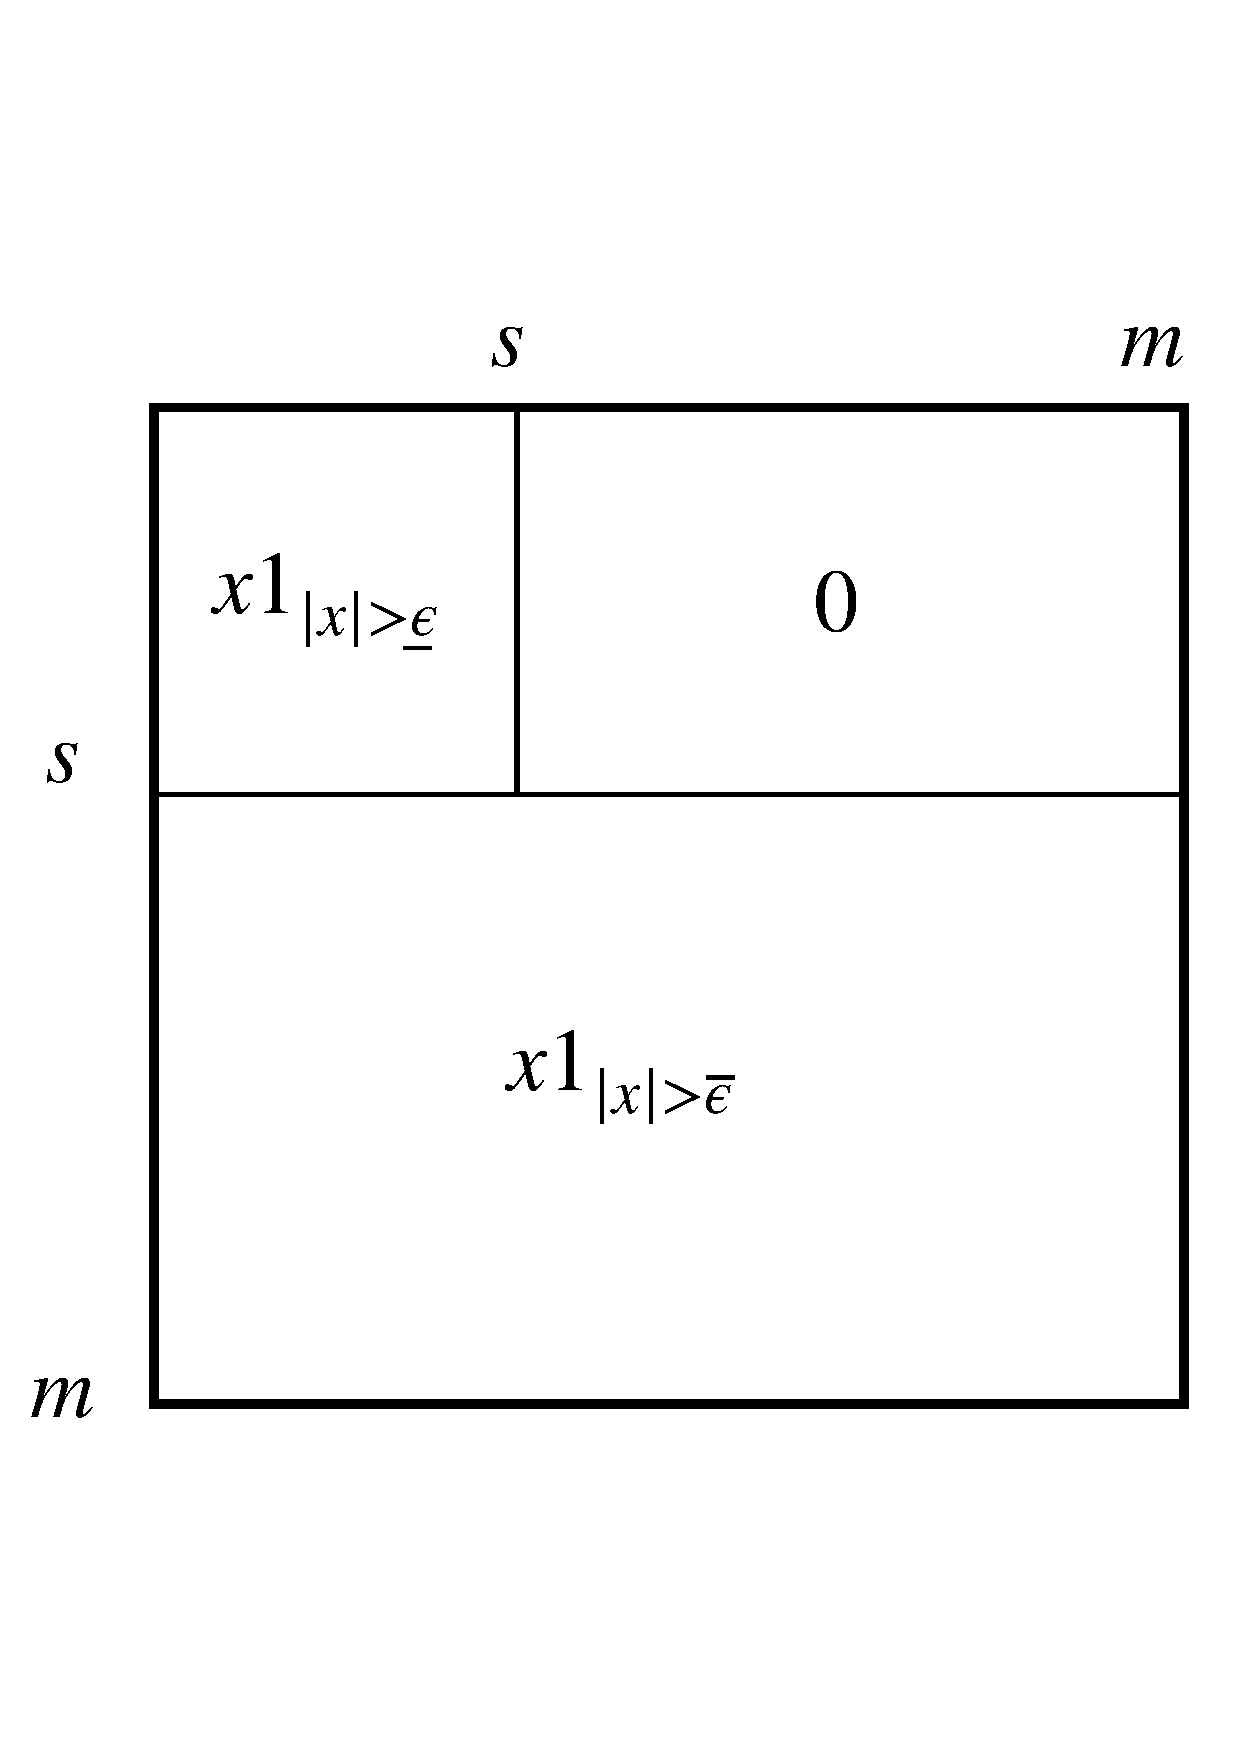
\includegraphics[scale=0.2]{fig_matrix.pdf}
    \mycaption{Adjency matrix A for the linear Gaussian framework}{Structure of matrix A in \eqref{eq:ex_lin} that is built using \eqref{eq:rules}.}
    \label{fig:matrix}
\end{figure}

To study the effect of the conditioning set on detecting the influences, in our experiments, we consider four different conditioning sets.
More precisely, to measure whether asset $i$ influences asset $j$, we estimate $I(X_i\rightarrow X_j||\mathcal{C}_j)$ for the following choices of the conditioning set:

\clearpage 

\begin{enumerate}
    \item \textit{True parents:} In this approach, we select $\mathcal{C}_j$ to be the true parents of $X_j$ excluding $X_i$, i.e., $\mathcal{C}_j=\mathcal{PA}_{j}\setminus\{X_i\}$.
    Note that this approach is not practical\footnote{This is because in structural learning problems, we do not know the true parents of each asset. In another words, if we had access to the true parents of each asset, we would have the DIG of the system and there is no need to compute the DIs.} and we use it only as the benchmark to better understand the performances of the other approaches. 
    
    \item \textit{Most correlated:} In this case, we define $\mathcal{C}_j$ to be the set of $k$ most correlated assets with $X_j$ (except $X_i$).
    
    \item \textit{Ideal portfolio:} In this scenario, $\mathcal{C}_j$ contains the portfolio $Q$, where $Q$ is defined in Lemma \ref{lemma:lin}.
    For further discussion see Appendix \ref{appendix2}. 
    %comprises of assets that influence $j$ except asset $i$, i.e., $\mathcal{C}_j=\{U\}$, where $Q=(Q_t)$ and $Q_t=\sum_{k\neq i}a_{i,k}X_{k,t}$.
    %Note that $Q$ coincides with the time series introduced in Lemma \ref{lemma:lin}. 
    
    \item \textit{RNN:} This method applies Algorithm \ref{alg} to estimate the time series $Q$ and defines $\mathcal{C}_j=\{Q\}$.
    
    %\item \textit{Maximally correlated:} In this case, $\mathcal{C}_j$ is the projection (ignoring i) maximally correlated with j (see Appendix C) \TODO{Do we really need this, because we have the ideal projection.}
\end{enumerate}
Note that we also applied the Koopman-based lifting techniques but due to its mentioned shortcomings, it was unable to robustly identify the interconnections. 
Hence, we could not compare its performance with the other methods. 
In this experiment, since the dynamics is linear and the noises are Gaussian, we use Equation \eqref{simueq} to estimate the DIs. 
Finally, we obtain the adjacency matrix of the corresponding DIGs by comparing the estimated DIs with a threshold $\alpha>0$, i.e., 
\begin{align}\label{eq:m}
    [\textbf{DIG}]_{j,i}=\left\{
\begin{array}{ll}
      1  & \text{if}\ \ \widehat{I}(X_i\rightarrow X_j||\mathcal{C}_j)>\alpha, \\
      0,  & \text{otherwise}, \\
\end{array} 
\right.
\end{align}
where $\widehat{I}(X_i\rightarrow X_j||\mathcal{C}_j)$ denotes the estimated DI from $X_i$ to $X_j$ given the conditioning set $\mathcal{C}_j$. 
In order to compare the performances of the aforementioned four approaches, we use the precision and recall measures between the true DIG (obtained from $\textbf{A}$) and their estimated DIGs. 
Formally, the precision and the recall are defined by
\begin{align*}
    Precision:= \dfrac{TP}{TP+FP}, \ \ Recall:= \dfrac{TP}{TP+FN},
\end{align*}
where 
\begin{align*}
    & TP := \sum_{i,j=1}^m 1_{a_{j,i} \neq 0}1_{ [\textbf{DIG}]_{j,i} \neq 0}, \ \ FP := \sum_{i,j=1}^m 1_{a_{j,i} = 0}1_{ [\textbf{DIG}]_{j,i} \neq 0},\\
    & FN := \sum_{i,j=1}^m 1_{a_{j,i} \neq 0}1_{ [\textbf{DIG}]_{j,i} = 0}.
    %\item $TN := \sum_{i,j=1}^m 1_{a_{j,i} = 0}1_{[\textbf{DIG}]_{j,i} \leq \alpha}$.
\end{align*}

\begin{figure*}[h]
        \centering
        \begin{subfigure}[b]{0.48\textwidth}
            \centering
            \includegraphics[width=\textwidth]{Linear_Performance_True parents.jpg}
        \end{subfigure}
        \quad
        \begin{subfigure}[b]{0.48\textwidth}  
            \centering 
            \includegraphics[width=\textwidth]{Linear_Performance_Most correlated assets.jpg}
        \end{subfigure}
        \vskip\baselineskip
        \begin{subfigure}[b]{0.48\textwidth}   
            \centering 
            \includegraphics[width=\textwidth]{Linear_Performance_Ideal Portfolio.jpg}
        \end{subfigure}
                  \quad
        \begin{subfigure}[b]{0.48\textwidth}   
            \centering 
            \includegraphics[width=\textwidth]{Linear_Performance_RNN.jpg}
        \end{subfigure}
        \mycaption{Precision and recall curves in the linear framework.}{Precision and recall curves for the \textit{true parents}, \textit{most correlated}, \textit{ideal portfolio}, and the \textit{RNN}, respectively.} 
        \label{perflin}
    \end{figure*}
    
Figure \ref{perflin} shows the performances of the four aforementioned approaches in the linear framework. 
%In a linear and Gaussian environment, the Gaussian estimator allows to compute the exact value of the DI. 
It is not surprising that the \textit{true parents} approach achieves 100\% accuracy, as it is anticipated by Lemma \ref{lemma:small}.
The \textit{ideal portfolio}'s performance is guaranteed by Lemma \ref{lemma:lin} and it is verified by our experiment.
However, it is important to emphasize that the \textit{ideal portfolio} shows ideal performance because the underlying model is linear. 
As we will see in the next section, its performance declines when the underlying model deviates from being linear. 
For the \textit{most correlated} approach, we used $k=10$ but as it is shown in Figure \ref{perflin}, it has the worst performance among the four conditioning methods. 
This is due to the fact that the set of the ten most correlated assets with a given asset $j$ does not necessarily contains the true parents of asset $j$.
On the other hand, we observe high accuracy from the \textit{RNN} approach which is a striking result.
This result is an evidence that a RNN is capable of estimating the ideal portfolio, i.e., the time series $Q$ in Lemma \ref{lemma:lin} without any side information about the underlying model. 


%On the other hand, the \textit{RNN} approach keeps its high performance even in non-linear system.  



\subsection{Non-Linear framework} \label{nonlinfr}
To compare the performances of the different approaches from the previous section in a non-linear environment, we simulate a set of quadratic processes whose dynamics is given below, 
\begin{equation}\label{eq:ex_non}
        X_{i,t} =b_i  {\textbf{X}^T_{t-1}} \textbf{A}_i \textbf{X}_{t-1} + N_{i,t}, \ i=1,...,m,
\end{equation}
where $\textbf{A}_i\in\mathbb{R}^{m \times m}$, $\textbf{X}_t = (X_{1,t}, X_{2,t},..., X_{m,t})^T$, $N_{i,t}\sim\mathcal{N}(0,\sigma^2)$, and $b_i\sim U(-0.9 , 0.9)$.
%Matrix  is associated to asset $i$. 
Note that the term $|[\textbf{A}_i]_{j,k} + [\textbf{A}_i]_{k,j}|$ captures the effect of $X_{j,t-1}X_{k,t-1}$ on $X_{i,t}$. Thus, it is possible to obtain the true parents of asset $i$ as follows,
\begin{equation}
 \mathcal{PA}_i = \{ X_j :  [\textbf{1}^T \cdot \big(|\textbf{A}^T_i + \textbf{A}_i|\big)]_{j}  > 0\},
\end{equation}
where $\textbf{1}$ denotes all-one vector of length $m$.
Each matrix $\textbf{A}_i$ is simulated independently by following the similar procedure as in Section \ref{linfr}.
In this experiment, since the model is non-linear, we could not apply \eqref{simueq} to estimate the DIs but instead we used the k-nearest method to estimate the mutual information and applied Equation \eqref{estdi}.
%sampling their entries randomly from a uniform distribution (similar to section \ref{linfr}).


Herein, we again compare the performances of the four different conditioning approaches. 
Figure \ref{fig:perfnonlin} shows the precision-recall curves for these approaches in the quadratic model with $m=15$. 
Precision-recall curves are a standard tools to illustrate and compare the performances of different learning methods. 
In this curve the precision is demonstrated in the y-axis vs. the recall on the x-axis for all potential values of the threshold $\alpha$. 

Similar to the linear setting, we use the \textit{true parents} as a benchmark since it has the ideal performance. 
It is however important to emphasize that this conditioning approach has higher complexity compared to the others. 
This is because in the \textit{true parent} approach, the size of the conditioning set is relatively larger than the other approaches. 

For the \textit{most correlated} approach, we use $k=5$, i.e., the size of the conditioning set is five.
With this method, we could slightly reduce the estimation complexity of the DIs compared to the  \textit{true parent} approach but this comes with the price of losing the performance.
Clearly, the performance of the \textit{most correlated} approach can be improved by increasing $k$ but this will increase the complexity.

The performance of the \textit{ideal portfolio} approach (using the time series in Lemma \ref{lemma:lin} as the conditioning) is worse than all others which is not surprising as the model is no longer linear. 
%\TODO{that is not the ideal portfolio, the ideal portfolio is not linear in the quadratic framework. that is the estimated linear portfolio using (31)}
This means that the information embedded in the linear portfolio is not sufficient to decide the non-linear influences among the time series. 

Finally, as it is shown in Figure \ref{fig:perfnonlin}, the \textit{RNN} approach outperforms the \textit{most correlated} and the \textit{ideal portfolio} approaches and it shows close performance to the \textit{true parents} but with the size of the conditioning set equal to one. 
This result once more fortifies our claim that with a RNN we can summarize the information of the network into one time series and use it for detecting the causal relationships. 
This claim is due to Lemma \ref{lemma:nonlinear} and the universal approximation theorem which states that a neural network with enough hidden layers can approximate any non-linear function (see \citet{HORNIK1989359}).
The slight difference between the performance of the \textit{RNN} and the \textit{true parents} is because of the estimation error in the recurrent neural network. 

%The latter result suggests that a one-dimension time series conditioning coming from the Neural Network is able to keep as much information as the N-dimensions conditioning coming from the True Parents. This is consistent with the Universal Approximation Theorem  (see ).  Complexity and computational time are also reduced; this reduction is growing as more and more assets are included in the DIG. 

\begin{figure}[h]
\centering
\includegraphics[width=0.75\textwidth]{precrecall_15assets.jpg}
\mycaption{Precision-recall curves for the quadratic model}{Blue, green, yellow and red lines show the precision-recall curve of the \textit{true parents}, \textit{most correlated}, \textit{ideal portfolio}, and the \textit{RNN}, respectively.}
\label{fig:perfnonlin}
\end{figure}

\subsection{Empirical DIG}

This section describes how to apply our approach to empirical data and obtain the DIG of US firms. 
We extracted the daily stock prices and the daily US Treasury rate as risk free returns from the CRSP database from 1990 to 2020. 
As the market is likely to evolve through these years, 
we chose to divide the dataset into six subsets, each of which has a length of five years and estimate the corresponding DIG of each subset separately. 
%chose to compute a different DIG for every five years. 
Herein, we assume that the causal structure of the market evolved but its rate was slow enough such that during a period of five years, the DIG of the market remained unchanged. 

For every subset, we keep the data of the 1000 firms with the highest maximum market capitalization and compute their excess return time series $X_{i,t}$, using the following relationship,
\begin{equation}
X_{i,t} = ln(P_{i,t}) - ln(P_{i,t-1}) - r_t,  
\end{equation}
where $P_{i,t}$ denotes the stock price of the firm $i$ at time $t$ and $r_{t}$ is the risk free rate at time $t$. 
Afterwards, we apply Algorithm \ref{alg} with the excess returns as the input to estimate the corresponding DIG of each subset. 
We use the k-nearest neighbor method to estimate the DIs.
We define the threshold $\alpha$ to be the unconditional mean across the estimated DIs. Note that in this experiment, the true DIGs of the market are not known, hence, we could not compute the precision-recall curves.

\clearpage

For the sake of presentation, instead of the complete DIGs with 1000 nodes, we draw the sub-graphs consisting of the 30 largest firms in Figures\footnote{For a better presentation, interactive plots are available at https://marcaureledivernois.github.io/firm-network/} \ref{empdig1}, \ref{empdig2}, and \ref{empdig3} . 
Each graph consists of 60 nodes illustrating the cause firm on the top hemisphere and the effect firm on the bottom hemisphere.
%Each hemisphere consists of 30 firms such that the north hemisphere denotes the cause and the south  shows all outdegrees of the 30 firms and the south hemisphere shows the indegrees of the 30 firms. 
For instance, if there is an edge between ``from: AAPL'' on the top and ``to: GOOGL'' on the bottom, it means that Apple influences Google. The dynamic evolution of the DIGs through time can often be explained by real events that happened in the market. For instance, in the DIG 2010-2014, Apple was not influencing General Electric (GE). However, on the 17th October 2017, Apple announced a partnership with GE to bring Predix, GE's data and analytics platform, to their iPhones and iPads. We are able to capture this partnership in the DIG 2015-2019 as an edge is now present from Apple to GE. Another example is the announced collaboration between AT\&T and Cisco to manage IoT devices and launch 5G service at the end of the 2010s: 
there was neither an edge from AT\&T to Cisco nor from  Cisco to AT\&T during the first half of the 2010s, but the DIG for the second half of the 2010s shows a mutual influence, reflecting an increased relationship between the two companies.

Table \ref{GrangerCausality} shows the Degree of Granger-Causality (DGC) defined as the fraction of relationships in the network among all potential relationships. Formally,
\begin{equation}
    DGC = \dfrac{1}{N^2} \sum_i \sum_j [\textbf{DIG}]_{j,i},
\end{equation}
These results show that the DGC increased both in the DotCom bubble and in the Subprime Crisis, suggesting an increase of the connectedness in turmoil periods. 
This finding is consistent with \citet{correlcrisis} stating that correlation increases in bear markets.

Tables \ref{outdegree} and \ref{indegree} show the outdegree and indegree of every firm in the six subsets. Outdegree is defined as the number of edges going out of a specific node. Indegree is the number of edges going to a specific node.
These tables also reveal interesting facts. For instance, the SPY ticker, an ETF launched in 1993 and aiming at tracking the S\&P500 return, enters in the 30 biggest market capitalizations in 2010 and has the highest number of outdegrees in the periods 2010-2014 and 2015-2019 but relatively low number of indegrees. This result suggests that the market return is influencing a high number of firms, but the converse is not necessarily true. 
%In each of the 5-years subsample, we use the excess returns of the 1000 biggest firms as conditional information to compute the DIs of the 30 biggest firms.
%\TODO{I dont understand the sample and subsample.}
%We used the k-nearest neighbor estimator to estimate the DIs and used algorithm \ref{alg} to  estimate the DIGs.  The threshold $\alpha$ is defined as the unconditional mean across the DIs.


\begin{table}[]
\centering
\begin{tabular}{cccccc}
\hline
\multicolumn{1}{|c|}{1990-1994} &
  \multicolumn{1}{c|}{1995-1999} &
  \multicolumn{1}{c|}{2000-2004} &
  \multicolumn{1}{c|}{2005-2009} &
  \multicolumn{1}{c|}{2010-2014} &
  \multicolumn{1}{c|}{2015-2019} \\ \hline
\multicolumn{1}{|c|}{0.23} &
  \multicolumn{1}{c|}{0.27} &
  \multicolumn{1}{c|}{0.18} &
  \multicolumn{1}{c|}{0.28} &
  \multicolumn{1}{c|}{0.32} &
  \multicolumn{1}{c|}{0.25} \\ \hline

\end{tabular}
\mycaption{Degree of Granger Causality (DGC) for each sub-graph.}{DGC is defined as the fraction of relationships in the network among all potential relationships.}
\label{GrangerCausality}
\end{table}

\begin{figure*}
        \centering
        \begin{subfigure}[b]{0.6\textwidth}
            \centering
            \includegraphics[width=\textwidth]{net1994.JPG}
        \end{subfigure}
        \vskip\baselineskip
        \begin{subfigure}[b]{0.6\textwidth}   
            \centering 
            \includegraphics[width=\textwidth]{net1999.JPG}
        \end{subfigure}
        \mycaption{Empirical DIG for the periods 1990-1994 and 1995-1999.}{Empirical DIG for the periods 1990-1994 (top) and 1995-1999 (bottom). Interactive graphs can be found at https://marcaureledivernois.github.io/firm-network/} 
        \label{empdig1}
    \end{figure*}
    
    
\begin{figure*}[]
        \centering
        \begin{subfigure}[b]{0.6\textwidth}
            \centering
            \includegraphics[width=\textwidth]{net2004.JPG}
        \end{subfigure}
        \vskip\baselineskip
        \begin{subfigure}[b]{0.6\textwidth}   
            \centering 
            \includegraphics[width=\textwidth]{net2009.JPG}
        \end{subfigure}
        \mycaption{Empirical DIG for the periods 2000-2004 and 2005-2009.}{Empirical DIG for the periods 2000-2004 (top) and 2005-2009 (bottom). Interactive graphs can be found at https://marcaureledivernois.github.io/firm-network/} 
        \label{empdig2}
    \end{figure*}
    
\begin{figure*}
        \centering
        \begin{subfigure}[b]{0.6\textwidth}
            \centering
            \includegraphics[width=\textwidth]{net2014.JPG}
        \end{subfigure}
        \vskip\baselineskip
        \begin{subfigure}[b]{0.6\textwidth}   
            \centering 
            \includegraphics[width=\textwidth]{net2019.JPG}
        \end{subfigure}
        \mycaption{Empirical DIG for the periods 2010-2014 and 2015-2019.}{Empirical DIG for the periods 2010-2014 (top) and 2015-2019 (bottom). Interactive graphs can be found at https://marcaureledivernois.github.io/firm-network/} 
        \label{empdig3}
    \end{figure*}    



\begin{table}[]
\resizebox{\textwidth}{!}{
\begin{tabular}{|ll|ll|ll|ll|ll|ll|}
\hline
\multicolumn{2}{|c|}{1990-1994} &
  \multicolumn{2}{c|}{1995-1999} &
  \multicolumn{2}{c|}{2000-2004} &
  \multicolumn{2}{c|}{2005-2009} &
  \multicolumn{2}{c|}{2010-2014} &
  \multicolumn{2}{c|}{2015-2019} \\ \hline
Ticker &
  Out &
  Ticker &
  Out &
  Ticker &
  Out &
  Ticker &
  Out &
  Ticker &
  Out &
  Ticker &
  Out \\ \hline
SBC  & 13 & JNJ  & 12 & XOM  & 12 & PEP  & 15 & SPY   & 17 & SPY   & 14 \\
CHV  & 11 & HWP  & 12 & JNJ  & 10 & WFC  & 13 & T     & 15 & DIS   & 12 \\
XON  & 10 & INTC & 12 & MSFT & 9  & CSCO & 12 & JNJ   & 15 & BRK   & 12 \\
PG   & 10 & BAC  & 12 & DELL & 9  & WMT  & 11 & CVX   & 13 & PFE   & 11 \\
GE   & 10 & PFE  & 11 & WMT  & 9  & IBM  & 11 & AAPL  & 12 & UNH   & 11 \\
AN   & 9  & IBM  & 11 & C    & 9  & PG   & 11 & INTC  & 12 & JPM   & 11 \\
BEL  & 9  & MSFT & 11 & HD   & 8  & CVX  & 11 & CSCO  & 12 & AAPL  & 10 \\
MRK  & 8  & SBC  & 11 & JPM  & 8  & HPQ  & 10 & GE    & 12 & GOOGL & 10 \\
IBM  & 8  & GE   & 10 & PFE  & 8  & VZ   & 10 & IBM   & 11 & WMT   & 9  \\
BMY  & 8  & MRK  & 10 & PG   & 7  & GE   & 9  & GOOGL & 11 & CSCO  & 9  \\
ABT  & 7  & LMG  & 9  & INTC & 7  & UBS  & 9  & XOM   & 11 & VZ    & 9  \\
AHP  & 7  & MO   & 9  & BAC  & 7  & PFE  & 9  & JPM   & 10 & BA    & 9  \\
T    & 7  & NT   & 9  & BMY  & 6  & C    & 9  & KO    & 10 & CVX   & 8  \\
BLS  & 7  & XOM  & 9  & SBC  & 6  & SLB  & 9  & MRK   & 10 & WFC   & 8  \\
AIG  & 7  & KO   & 9  & IBM  & 5  & MSFT & 9  & BRK   & 10 & V     & 8  \\
F    & 7  & HD   & 8  & TWX  & 5  & ORCL & 9  & SLB   & 10 & PG    & 8  \\
HWP  & 7  & BEL  & 8  & AIG  & 5  & MRK  & 8  & WMT   & 10 & T     & 7  \\
MOT  & 7  & BMY  & 8  & CSCO & 4  & KO   & 8  & VZ    & 9  & JNJ   & 7  \\
DD   & 6  & SUNW & 8  & GE   & 4  & GOOG & 7  & DIS   & 9  & MRK   & 7  \\
DIS  & 6  & AIG  & 7  & VZ   & 4  & XOM  & 7  & PFE   & 9  & KO    & 6  \\
MOB  & 6  & WCOM & 7  & MRK  & 4  & JNJ  & 7  & BAC   & 8  & XOM   & 5  \\
PEP  & 6  & CSCO & 6  & MOT  & 4  & MO   & 7  & PM    & 8  & MSFT  & 5  \\
MSFT & 6  & QCOM & 6  & TXN  & 4  & JPM  & 6  & ORCL  & 7  & MA    & 5  \\
INTC & 6  & C    & 6  & HPQ  & 3  & COP  & 6  & PG    & 7  & BABA  & 5  \\
WMT  & 6  & PG   & 6  & ORCL & 3  & T    & 6  & PEP   & 6  & FB    & 4  \\
GTE  & 5  & DELL & 5  & KO   & 2  & INTC & 6  & MSFT  & 6  & BAC   & 4  \\
MO   & 5  & ORCL & 4  & SUNW & 1  & AAPL & 6  & C     & 5  & INTC  & 4  \\
JNJ  & 4  & WMT  & 4  & LU   & 1  & BAC  & 5  & WFC   & 5  & GE    & 3  \\
PFE  & 4  & EMC  & 2  & EMC  & 0  & MT   & 4  & AMZN  & 5  & HD    & 3  \\
KO   & 2  & AOL  & 2  & NT   & 0  & AIG  & 4  & GILD  & 5  & AMZN  & 2  \\ \hline
\end{tabular}}
\mycaption{Outdegrees ranked for each sub-graph.}{Outdegree (Out) is defined as the number of edges going out of a specific node.}
\label{outdegree}
\end{table}




\begin{table}[]
\resizebox{\textwidth}{!}{
\begin{tabular}{|ll|ll|ll|ll|ll|ll|}
\hline
\multicolumn{2}{|c|}{1990-1994} &
  \multicolumn{2}{c|}{1995-1999} &
  \multicolumn{2}{c|}{2000-2004} &
  \multicolumn{2}{c|}{2005-2009} &
  \multicolumn{2}{c|}{2010-2014} &
  \multicolumn{2}{c|}{2015-2019} \\ \hline
Tic  & In & Tic  & In & Tic  & In & Tic  & In & Tic   & In & Tic   & In \\ \hline
XON  & 22 & BEL  & 15 & MOT  & 12 & MRK  & 19 & MRK   & 18 & UNH   & 17 \\
CHV  & 17 & JNJ  & 15 & INTC & 11 & ORCL & 19 & PM    & 15 & PFE   & 16 \\
AN   & 13 & AOL  & 14 & C    & 11 & BAC  & 16 & JPM   & 15 & HD    & 14 \\
SBC  & 12 & XOM  & 14 & SUNW & 11 & SLB  & 14 & ORCL  & 14 & AMZN  & 14 \\
HWP  & 11 & NT   & 12 & ORCL & 10 & WFC  & 13 & IBM   & 14 & GOOGL & 12 \\
PEP  & 10 & QCOM & 12 & BMY  & 9  & JPM  & 12 & XOM   & 13 & GE    & 12 \\
AHP  & 10 & SUNW & 11 & DELL & 9  & COP  & 12 & PG    & 13 & PG    & 12 \\
MOB  & 10 & ORCL & 11 & TWX  & 7  & MT   & 11 & JNJ   & 12 & CVX   & 11 \\
GTE  & 9  & CSCO & 11 & HPQ  & 7  & PEP  & 10 & DIS   & 12 & BABA  & 9  \\
IBM  & 9  & C    & 11 & GE   & 7  & C    & 10 & INTC  & 11 & MRK   & 9  \\
BMY  & 8  & DELL & 10 & CSCO & 7  & MO   & 10 & WFC   & 10 & DIS   & 9  \\
ABT  & 8  & SBC  & 10 & LU   & 6  & CVX  & 10 & C     & 10 & WFC   & 8  \\
KO   & 7  & BMY  & 9  & HD   & 6  & AIG  & 9  & VZ    & 10 & BA    & 7  \\
BEL  & 7  & WCOM & 9  & TXN  & 6  & T    & 9  & WMT   & 10 & MA    & 7  \\
MSFT & 7  & GE   & 9  & EMC  & 6  & JNJ  & 8  & GE    & 10 & AAPL  & 7  \\
BLS  & 6  & IBM  & 9  & BAC  & 5  & GOOG & 7  & KO    & 9  & T     & 7  \\
PFE  & 6  & MO   & 9  & PG   & 5  & KO   & 7  & BAC   & 9  & WMT   & 6  \\
DD   & 6  & LMG  & 8  & WMT  & 5  & VZ   & 6  & PFE   & 9  & MSFT  & 6  \\
JNJ  & 5  & HWP  & 6  & VZ   & 5  & MSFT & 6  & AAPL  & 9  & INTC  & 6  \\
WMT  & 4  & MSFT & 6  & JPM  & 4  & INTC & 6  & SPY   & 8  & FB    & 5  \\
F    & 4  & BAC  & 5  & KO   & 3  & AAPL & 6  & CVX   & 7  & KO    & 5  \\
MRK  & 4  & INTC & 5  & NT   & 3  & GE   & 6  & AMZN  & 7  & JPM   & 4  \\
PG   & 4  & WMT  & 5  & XOM  & 2  & WMT  & 6  & GILD  & 7  & XOM   & 4  \\
AIG  & 4  & PFE  & 4  & MSFT & 2  & XOM  & 5  & CSCO  & 7  & JNJ   & 4  \\
T    & 3  & AIG  & 4  & AIG  & 2  & PFE  & 5  & GOOGL & 7  & SPY   & 4  \\
GE   & 2  & KO   & 3  & MRK  & 1  & CSCO & 4  & MSFT  & 6  & BRK   & 4  \\
MO   & 2  & MRK  & 2  & PFE  & 1  & HPQ  & 4  & PEP   & 5  & CSCO  & 3  \\
INTC & 2  & PG   & 2  & SBC  & 1  & UBS  & 2  & SLB   & 5  & BAC   & 2  \\
DIS  & 1  & HD   & 2  & IBM  & 0  & IBM  & 1  & T     & 4  & V     & 1  \\
MOT  & 1  & EMC  & 1  & JNJ  & 0  & PG   & 1  & BRK   & 4  & VZ    & 1  \\ \hline
\end{tabular}}
\mycaption{Indegrees ranked for each sub-graph.}{Indegree (In) is defined as the number of edges going to a specific node.}
\label{indegree}
\end{table}

\section{Conclusion}\label{sec:con}

In this chapter, we introduce an information-theoretic measure known as directed information that is capable of capturing nonlinear Granger-causality in an interactive system. 
We develop a novel algorithm based on recurrent neural network utilized with directed information. 
This algorithm can infer the interconnections within a large network with less complexity than previous works. As a proof of concept, we show that our approach performs well both in a linear and in a non-linear simulated environments. Finally, we apply this algorithm to infer the causal relationships among the major US firms during 1990 to 2020. 

 
 




